\documentclass[a4paper,11pt,fleqn]{article}%fleqn pour aligner les equations à gauche
\usepackage{/home/rweye/Nextcloud/Documents/Overleaf/Styles/Cours}

\newcommand{\chnum}{Chapitre 1}
\newcommand{\chtitle}{La découverte de la radioactivité et du radium}
\newcommand{\dtype}{Activité 3}


\begin{document}
\maketitle

%Les découvertes de la radioactivité et du radium, couronnées par le prix Nobel de physique en 1903, révolutionnent physique, chimie, mais aussi médecine, armement et énergie.
\section{Faire le lien entre radioactivité et rayons X}
\begin{figure}[h!]
    \begin{minipage}{.27\linewidth}
        \begin{minipage}{\linewidth}
            \caption{Découverte de la radioactivité}
            \centering
            
\includegraphics[width=.6\linewidth]{Ressources/1ES_Act2_QR1.png}
        \end{minipage}\vspace{1em}
        \begin{minipage}{\linewidth}
        		\caption{Plaque photographique}
        		\begin{center}
        			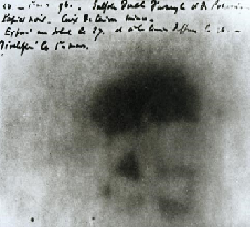
\includegraphics[width=.8\linewidth]{Ressources/1ES_Act2_Fig1.png}
        		\end{center}
            Impression laissée par le rayonnement radioactif et notes manuscrites de Becquerel.
        \end{minipage}\vspace{1em}
        \begin{minipage}{\linewidth}
            \caption{Henri Becquerel Physicien français (1852-1908)}
            \begin{center}
            		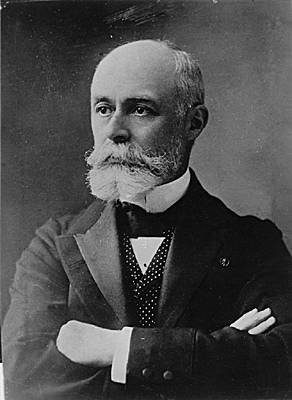
\includegraphics[width=.6\linewidth]{Ressources/1ES_C1_Act2_Becquerel.jpg}
            \end{center}
            En cherchant les raisons de la phosphorescence (rayonnement émis par certaines substances), il découvre la radioactivité naturelle et les rayons "uraniques".
        \end{minipage}
    \end{minipage}\hspace{.015\linewidth}\vline\hspace{.015\linewidth}
    \begin{minipage}{.7\linewidth}
        \begin{minipage}{.46\linewidth}
            \caption{Radiographie de la main gauche de Madame Röntgen}
            \begin{center}
            		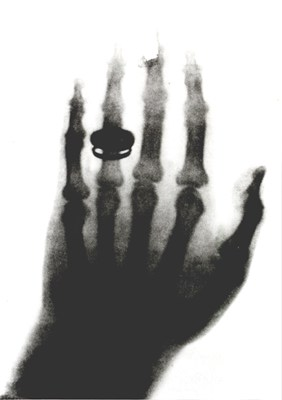
\includegraphics[width=.75\linewidth]{Ressources/1ES_C1_Act2_Röntgen.jpg}
            \end{center}
            En 1895, le physicien allemant Wilhelm Röntgen (1845-1923) découvre les rayons X et obtient le premier prix Nobel de physique en 1901.
        \end{minipage}\hspace{.06\linewidth}
        \begin{minipage}{.5\linewidth}
        \caption{Protocole de Becquerel}Parmi les expériences qui précèdent, quelques-unes avaient été préparées le mercredi 26 et le jeudi 27 février et, comme ces jours-là, le Soleil ne s'est montré que d'une manière intermittente, j'avais conservé les expériences toutes préparées et rentré les châssis à l'obscurité dans le tiroir d'un meuble, en laissant en place les lamelles du sel d'uranium. Le soleil ne s'étant pas montré de nouveau les jours suivants, j'ai développé les plaques photographiques le 1 mars, en m'attendant à trouver des images très faibles. Les silouettes apparurent, au contraire, avec une grande intensité.
        \begin{flushright}
            "Sur les radiations invisibles émises par les corps phosphorencents", \textit{Comptes rendus de l'Académie des sciences, 1896.}
        \end{flushright}
        \end{minipage}\vspace{3.75em}
        \begin{minipage}{\linewidth}
            \caption{Marie Sktodowska-Curie, physicienne et chimiste française d'origine polonaise (1867-1934) et Pierre Curie, physicien français (1959-1906)}
            \begin{center}
                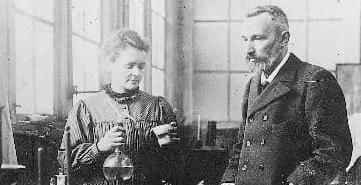
\includegraphics[width=.75\linewidth]{Ressources/1ES_C1_Act2_Couple Curie.jpg}
            \end{center}
            Travaillant en tandem, ils explorent la radioactivité afin d'expliquer le phénomène. Ils découvrent deux éléments : le polonium et le radium sous forme ionique. Marie Curie est considérée comme la première femme reconnue par la communauté scientifique internationale.
        \end{minipage}
    \end{minipage}    
\end{figure}

\section{Découvrir les propriétés du radium}
\begin{figure}[h!]
	\begin{minipage}{.37\linewidth}
	\caption{Impact du gaz radon dans les bâtiments}
	\begin{center}
        
\includegraphics[width=.45\linewidth]{Ressources/1ES_Act2_QR2.png}
    \end{center}
	Le gaz radon est issu de la désintégration de l'uranium et du radium.
	\end{minipage}\hspace{.03\linewidth}
	\begin{minipage}{.6\linewidth}
	\caption{Application et utilisations du radium}
	Métal aujourd'hui oublié, le radium fit  sensation lors de sa découverte. Le nouvel élément était rare et cher, spontanément lumineux, et, il émettait une quantité prodigieuse de rayonnement et d'énergie : 1,4 million de fois celle de l'uranium découvert par Becquerel. C'était le plus radioactif des éléments que l'on pouvait voir et peser.\\
	Les rayonnements du radium devinrent un formidable outil pour l'exploration de la structure microscopique de la matière. Les applications de la médecine commencèrent dès la fin de 1901. Un nouveau domaine fut créé pour regrouper toutes les applications thérapeutiques où le radium est présent : la curithérapie ou radiumthérapie.
	\end{minipage}
	
	\vspace{1em}
	\begin{minipage}{.57\linewidth}
	\caption{Attribution des prix Nobel}
	\textbf{Bobel Prize in Physics 1903 :}\\
	To Henri Becquerel, "in recognition of the extraordinary services he has rendered by his discovery os spontaneous radioactivity".\\
	To Marie and Pierre Curie, "in recognition of the extraordinary services they have rendered by their joint researches on the radiation phenomena discovered by Professor Henri Becquerel."\\
	\vspace{1em}
	
	\textbf{Nobel Prize in Chemistry 1911 :}\\
	To Marie Curie, "in recognition of her services to the advancement of chemistry by the discovery of the elements radium and polonium, by the isolation od radium and the study of the nature and compounds of this remarkable element."\\
	\begin{flushright}
	D'après \textit{www.nobelprize.org}
	\end{flushright}
	\end{minipage}\hspace{0.03\linewidth}
	\begin{minipage}{.4\textwidth}
	\caption{Le radium métallique}
    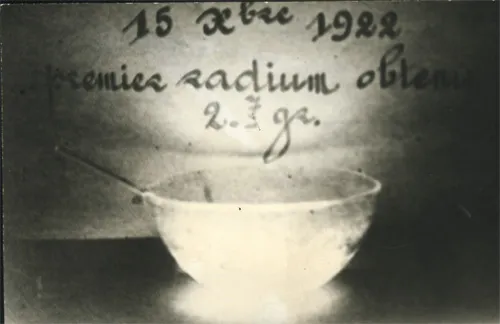
\includegraphics[width=\linewidth]{Ressources/1ES_Act2_Fig3.png}
	En 1910, Marie Curie et André Debierne (chimiste français 1874-1949) isolent et caractérisent le radium métallique. Le radium émet naturellement, spontanément, de la lumière.
	\end{minipage}
	
	\vspace{1em}
	\begin{minipage}{.37\linewidth}
		\caption{Campagne de publicité mensongère combattue par Marie Curie}
		\centering
    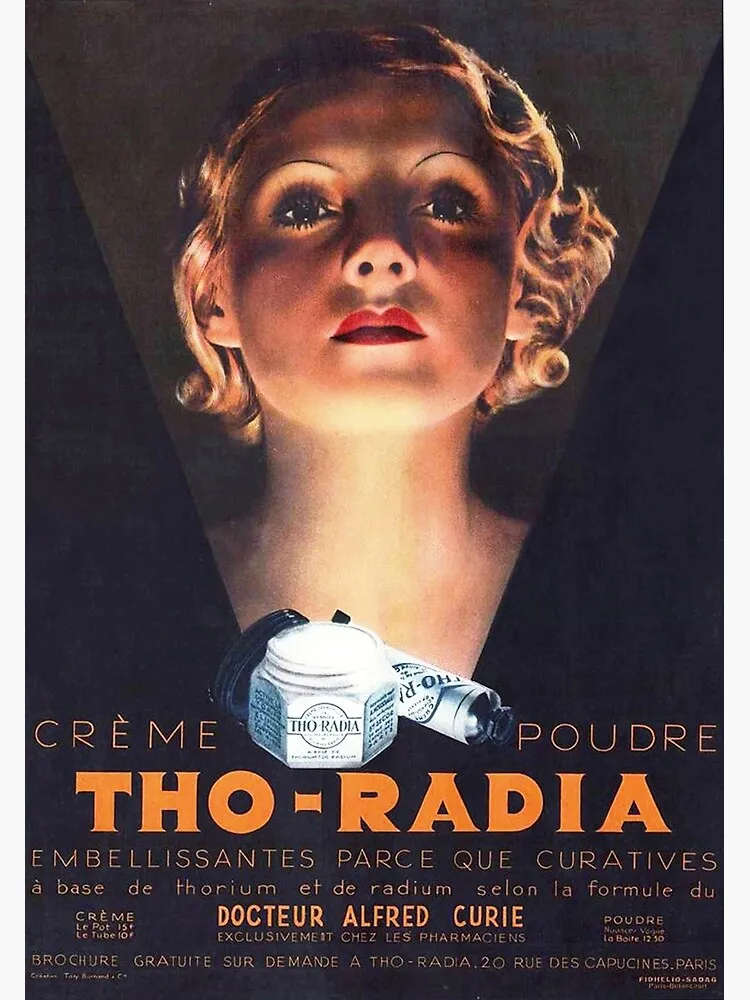
\includegraphics[width=.75\linewidth]{Ressources/1ES_Act2_Fig4.png}
	\end{minipage}\hspace{0.03\linewidth}
	\fcolorbox{blue!15}{blue!15}{\begin{minipage}{.6\linewidth}
		\textbf{Questions :}
\begin{enumerate}
	\item Relever les grandes étapes de la découverte du radium et de la radioactivité. Est-il si aisé d'attribuer la parenté d'une découverte scientifique ?
	\item Présenter les caractéristiques du radium, ses utilisations et les conséquences possibles de l'utilisation d'un produit radioactif.
	\item Élaborer une affiche décrivant les circonstances historiques et scientifiques propices à la découverte de la radioactivité et du radium.
\end{enumerate}
	\vspace{2cm}
	\end{minipage}}
\end{figure}


\end{document}
